\clearpage
\twocolumn[{%
\subsection{Size generalisation to 3B}
\label{app:rq10_size_generalisation}

\noindent\begin{minipage}[t]{0.485\textwidth}
\vspace{0pt}
\paragraph{Research Question.} \emph{Does a ranking that holds at 1.7B still hold one rung above it, at 3B?}

\paragraph{Setup.} The deep cells trained at 3B (seed 1904) and the same families at 1.7B. Each (family, task) is scored at both rungs. Left: for each benchmark, the share of its tasks above chance at 1.7B and at 3B. We show the benchmarks with at least five tasks whose share moves. Right: DA-size from the final checkpoints of 90M--1B to the 3B final checkpoint and to the 1.7B final checkpoint, on the same single-axis decisions. Benchmark accuracy (tasks above chance at the proxy, at 1.7B and at 3B) and per-language bits per byte are pooled separately. The bands are 90\% leave-one-family-out jackknife bands.
\end{minipage}\hfill
\begin{minipage}[t]{0.485\textwidth}
\vspace{0pt}
\begin{rqfinding}
\textbf{1. The 3B rung measures more than the reference but decides no differently.} On the same six families it lifts the above-chance count from 522 to 687 of 841 tasks (+32 \%), while mono-axis DA-size on identical decisions stays at 0.49--0.54 in benchmark accuracy (bBPB twins pooled) to either reference and at 0.81--0.96 in per-language BPB. (Figure~\ref{fig:app_rq10_size_generalisation}.)
\\
\\
\textbf{2. In benchmark accuracy no proxy predicts the 3B decision, the 1.7B reference included.} On the six families' gated benchmark tasks (the bBPB twins left out), DA-size $\rightarrow$ 3B is 0.47--0.52 mono-axis over 164--258 tasks and 0.48--0.53 multi-axis over 189--303.
\\
\\
\textbf{3. The ``same families'' column is not benchmark-only, and neither is the 3B column.} Its 0.52--0.53 mono-axis and 0.53--0.54 multi-axis pool the bBPB twins, which exist at 1.7B on all six families and at 3B on five (panel (a)'s dashed lines rest on a median of 622 and 728 tasks against 501 and 556 to 3B).
\end{rqfinding}
\end{minipage}

\vspace{\baselineskip}
\noindent\begin{minipage}{\textwidth}
\centering
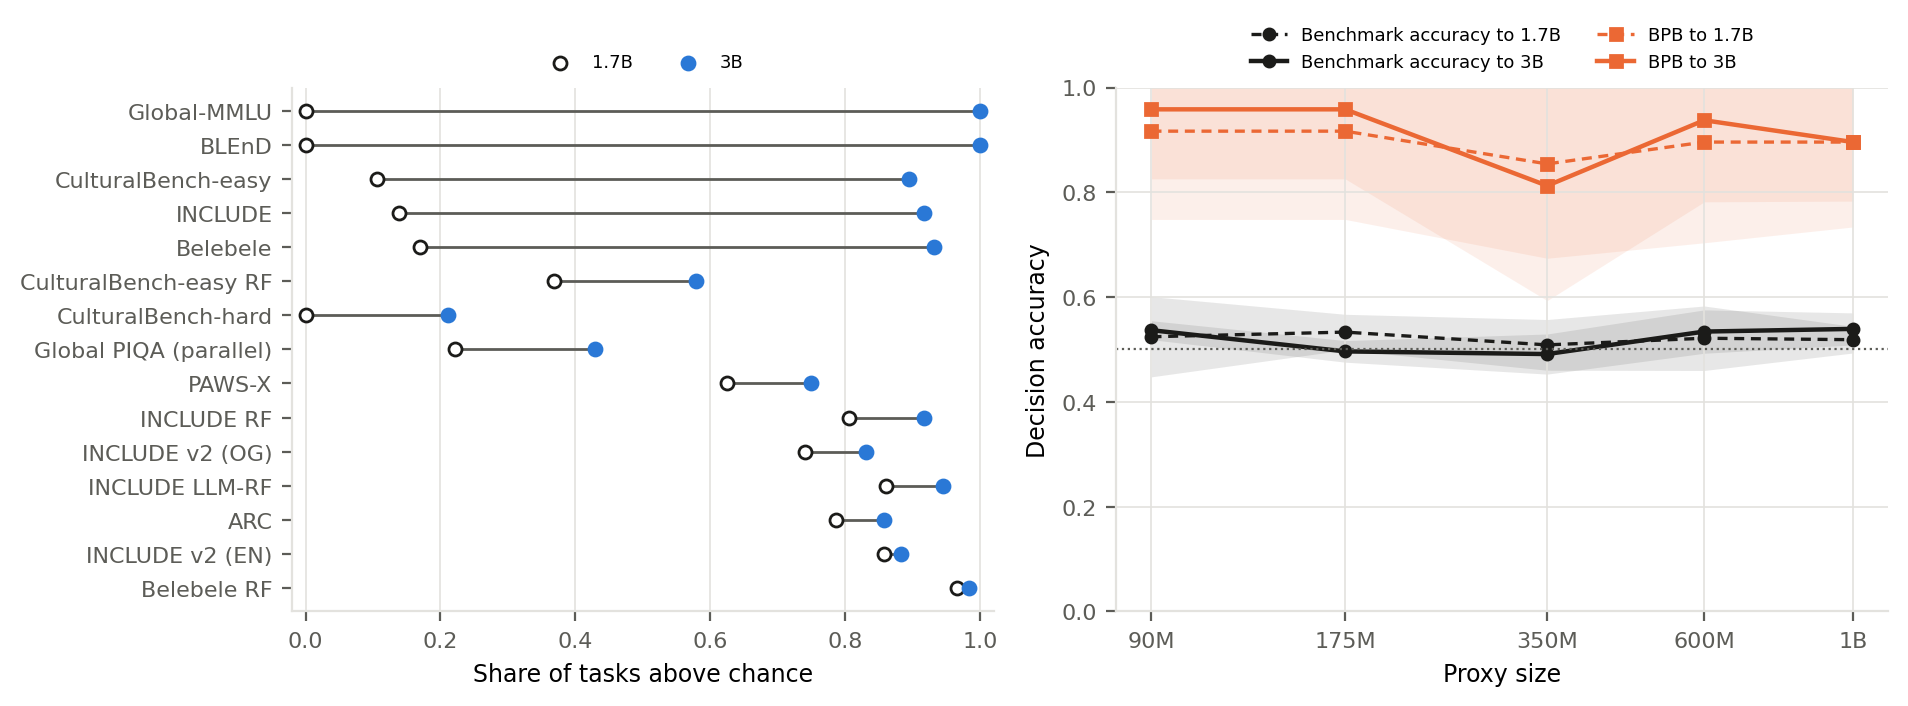
\includegraphics[width=\textwidth,height=0.36\textheight,keepaspectratio]{figures/app_rq10_size_generalisation.png}
% source: src/signal-and-noise/analysis/rq10_size_generalisation/pretraining/predictivity/gate_share_and_da_size_mono_axis_paper.png
\captionof{figure}{\textbf{The 3B rung measures more than the reference but decides no differently.} Left: for each benchmark with at least five tasks whose share moves, the share of its tasks above chance at 1.7B (open circles) and at 3B (filled circles). Right: DA-size of the proxies 90M--1B against the 3B final checkpoint (solid) and against the 1.7B final checkpoint (dashed), on benchmark accuracy (black) and on per-language bits per byte (orange). The bands are 90\% leave-one-family-out jackknife bands and the dotted line marks 0.5.}
\label{fig:app_rq10_size_generalisation}
\end{minipage}
\vspace{\baselineskip}
}]
